\subsection{Problem 2: Regression Analysis of Heating Oil Usage}
\subsubsection{Problem Description}
Develop a model for estimating heating oil used for a single-family home in January based on average temperature and amount of insulation in inches.

\begin{table}[h!]
\centering
\begin{tabular}{c|c|c}
Oil & Temp F & Insulation \\
\hline
270 & 40 & 4 \\
362 & 27 & 4 \\
162 & 40 & 10 \\
45 & 73 & 6 \\ 
91 & 65 & 7 \\
233 & 65 & 40 \\
372 & 10 & 6 \\
305 & 9 & 10 \\
234 & 24 & 10 \\
122 & 65 & 4 \\
25 & 66 & 10 \\
210 & 41 & 6 \\
450 & 22 & 4 \\
325 & 40 & 4 \\
52 & 60 & 10 \\
\hline
\end{tabular}
\end{table}
\subsubsection{Simulation Analysis}
\textbf{(a) Model Fitting and $R^2$ Comparison}
We fit linear and quadratic models and compute $R^2$:

\begin{figure}[H]
    \centering
    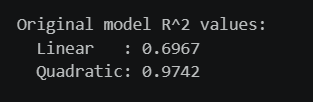
\includegraphics[height=0.15\textwidth]{figures/P2 orig.png}
    \caption{R-squared values for the original data}
    \label{fig:originalr2p2}
\end{figure}

\textbf{Observation:}  
The quadratic model $R^2$ value is higher than the linear model. The quadratic model fits the data better, but this judgement is affected by the outliers, so it is unreliable.

\textbf{Conclusion:}  
Although the quadratic model has the highest $R^2$, we can't tell if it adequately capture the data behavior.


\vspace{.4cm}
\textbf{(b) Outlier Removal and Re-fitting}
the point $(Insulation=400)$ is clearly outside the general trend and is treated as an outlier.

Recomputing the models:

\begin{figure}[H]
    \centering
    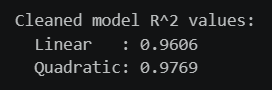
\includegraphics[height=0.15\textwidth]{figures/P2 clean.png}
    \caption{R-squared values for cleaned data}
    \label{fig:cleanr2p2}
\end{figure}

\textbf{Conclusion:}  
The linear model already provides an excellent fit. Higher-order models offer only marginal improvement and introduce unnecessary complexity.

\[
\boxed{\text{Best model: Linear}}
\]

\vspace{.4cm}
\textbf{(c) Prediction for temperature $15^\circ$F and insulation 5 inches}

For temperature $15^\circ$F and insulation 5 inches:
\begin{figure}[H]
    \centering
    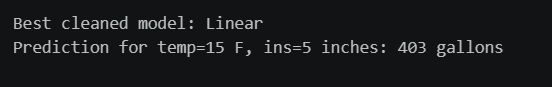
\includegraphics[height=0.15\textwidth]{figures/P2 pred.png}
    \caption{Best cleaned model and prediction for temperature $15^\circ$F with insulation 5 inches}
    \label{fig:p2_prediction_oil}
\end{figure}

\textbf{Final Interpretation:}  
The presence of the outlier significantly degrades model performance. After removing it, the data is well-described by a linear model, which provides a reliable prediction for future values.